\section{Ergebnisse}
\subsection{Laufbandversuch}
Die beste Übereinstimmung für Periodendauer und Frequenz werden für inverses Pendel und Schwerkraftpendel bei 2~km~h$^{-1}$ erreicht. Dabei wird die Periodendauer durch das inverse Pendel unterschätzt (-2,9~\%) und durch das Schwerkraftpendel überschätzt (5,1~\%). Die Abweichungen der Frequenz liegen bei 3,0~\% für inverses Pendel und -4,8~\% für das Schwerkraftpendel. Die geringste Anstrengung wurde bei einer Geschwindigkeit von 3~km~h$^{-1}$ wahrgenommen.

\begin{table}[h!]
\centering
\caption[Ergebnisse Laufbandversuch]{Periodendauer~P und Frequenz~F für einen Doppelschritt bei sieben Geschwindigkeiten. Inverses Pendel (P$_{inv}$, F$_{inv}$) und Schwerkraftpendel (P$_{schw}$, F$_{schw}$) sowie Abweichung in \%.}
\label{tab:Erg_Pend}
\begin{tabular}{c c c c c c c c c c c}
\toprule
Geschw. & Wertung & $P_{inv}$ & Abw. & $F_{inv}$ & Abw. & $P_{schw}$ & Abw. & $F_{schw}$ & Abw. & Schritt-\\
$[km~h^{-1}]$  & [1-10] & [T] & $[\%]$ & [Hz] & $[\%]$ &  [T] & $[\%]$ & [Hz] & $[\%]$ & länge [m]\\
\midrule
Pendel	&---& 1,36 	& ---	& 0,74 	& ---	& 1,90	&---	& 0,52&	---		& ---	\\
1 		& 8	& 1.68 	& 23,6	& 0,60 	&  -19,1& 4,16	& 118,6	& 0,24&	-54,3	& 0,51	\\
2 		& 5 & 1.32 	& -2,9	& 0,76 	&  3,0	& 2,00	& 5,1 	& 0,5 &	-4,8	& 0,54	\\
3 		& 1 & 1.16 	& -14,7	& 0,86 	& 17,2	& 1,44	& -24,3	& 0,69&	32,2	& 0,65	\\
4 		& 3 & 1,00	& -26,4	& 1,00 	& 35,9	& 1,28	& -32,7	& 0,78&	48,7	& 0,73	\\
5 		& 3 & 0.92 	& -32,3	& 1,09 	& 47,7	& 1,12	& -41,2	& 0,89&	69,9	& 0,79	\\
6 		& 5 & 0.88 	& -35,3	& 1,14 	& 54,5	& 1,04	& -45,4	& 0,96&	83,0	& 0,86	\\
7 		& 10& 0.84 	& -38,2	& 1,19 	& 61,8	& 0,92	& -51,7	& 1,09&	106,7	& 0,9	\\
\bottomrule
\end{tabular}
\end{table}

\subsection{Laufstreckenversuch}
Der Vergleich der Bodenreaktionskräfte bei 2, 5 und 7~km~h$^{-1}$ zeigt mit steigender Geschwindigkeit ein Ansteigen der Kraftmaxima und Sinken der -minima bei kürzeren Standphasen (s.~\autoref{fig:res_Kraefte}). Alle drei Kurven zeigen einen kurzen Einbruch des Anstiegs vor dem ersten Maximum. Für 2~km~h$^{-1}$ liegt dieses Maximum bei 93\% des Körpergewichts. Bis auf ein Minimum kurz nach dem Maximum bleibt die Belastung nahezu konstant bis zum Abfallen der Kurve. Für 5~km~h$^{-1}$ liegt das erste Maximum bei 103\% des Körpergewichts, sinkt auf 70\% ab und stiegt erneut auf 109\% an. Für 7~km~h$^{-1}$ liegt das erste Maximum bei 125\%, das Minimum bei 59\% und das zweite Maximum bei 101\%.\\

\begin{figure}[h!]
	\centering
	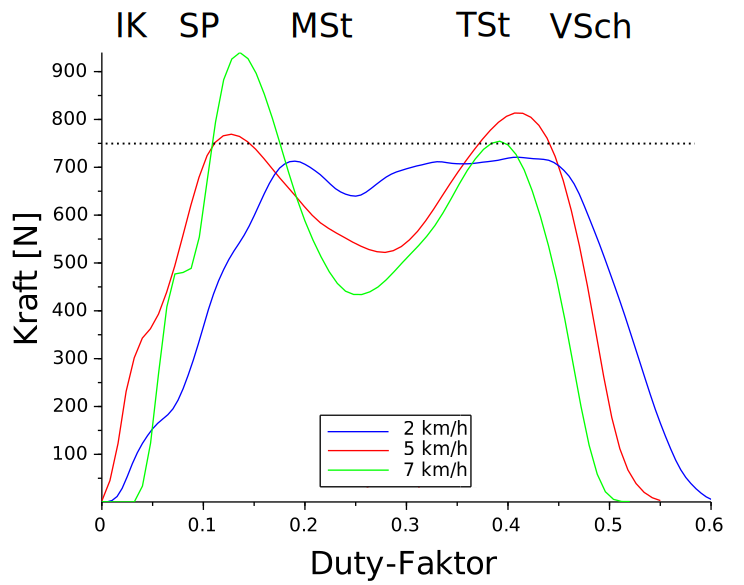
\includegraphics[width=0.7\linewidth]{bilder/Ergebnisse/BRK}
	\caption[Bodenreaktionskräfte]{Vergleich der Bodenreaktionskräfte auf der Laufstrecke bei 2, 5 und 7~km~h$^{-1}$. Gestrichelte Linie stellt das Körpergewicht dar. Standphasen: Initialer Kontakt IK, Stoßdämpfungsphase SP, mittlere und terminale Standphase MSt bzw. TSt sowie Vorschwungphase VSch}
	\label{fig:res_Kraefte}
\end{figure}

Die Kräfte in X-Richtung zeigen in allen Gelenken in der initialen Kontaktphase kurz Werte in Laufrichtung auf, welche mit der Stoßdämpfungsphase entgegen der Laufrichtung wirken. Während der mittleren Standphase wirkt die Kraft wieder in Laufrichtung mit einem Maximum zu Beginn der terminalen Standphase. Der Verlauf der Kräfte in Y-Richtung spiegelt den Verlauf der Bodenreaktionskräfte wieder, jedoch wirkt die Kraft hier in entgegengesetzte Richtung. Der Verlauf der Momente ändert sich erheblich von Gelenk zu Gelenk. Während das Moment im Knöchel während des initialen Kontakts fast bei Null ist, wird es mit Beginn der Stoßdämpfungsphase positiv und bleibt relativ konstant bis zum Ende der terminalen Standphase. In der Vorschwungphase ist es auf Null abgesunken. Im Knie werden wesentlich kleinere Momente er-reicht, welche um Null schwanken. Das Maximum trifft mit dem Beginn der Stoßdämpfungsphase zusammen, sinkt dann während der mittleren Standphase auf Null und wird leicht negativ mit der terminalen Standphase. Der Verlauf des Momentes in der Hüfte ähnelt dem im Knie, ist jedoch deutlich stärker ausgeprägt und zeigt in der Stoßdämpfungsphase starkes Rauschen.\\
\begin{figure}[h!]
	\centering
	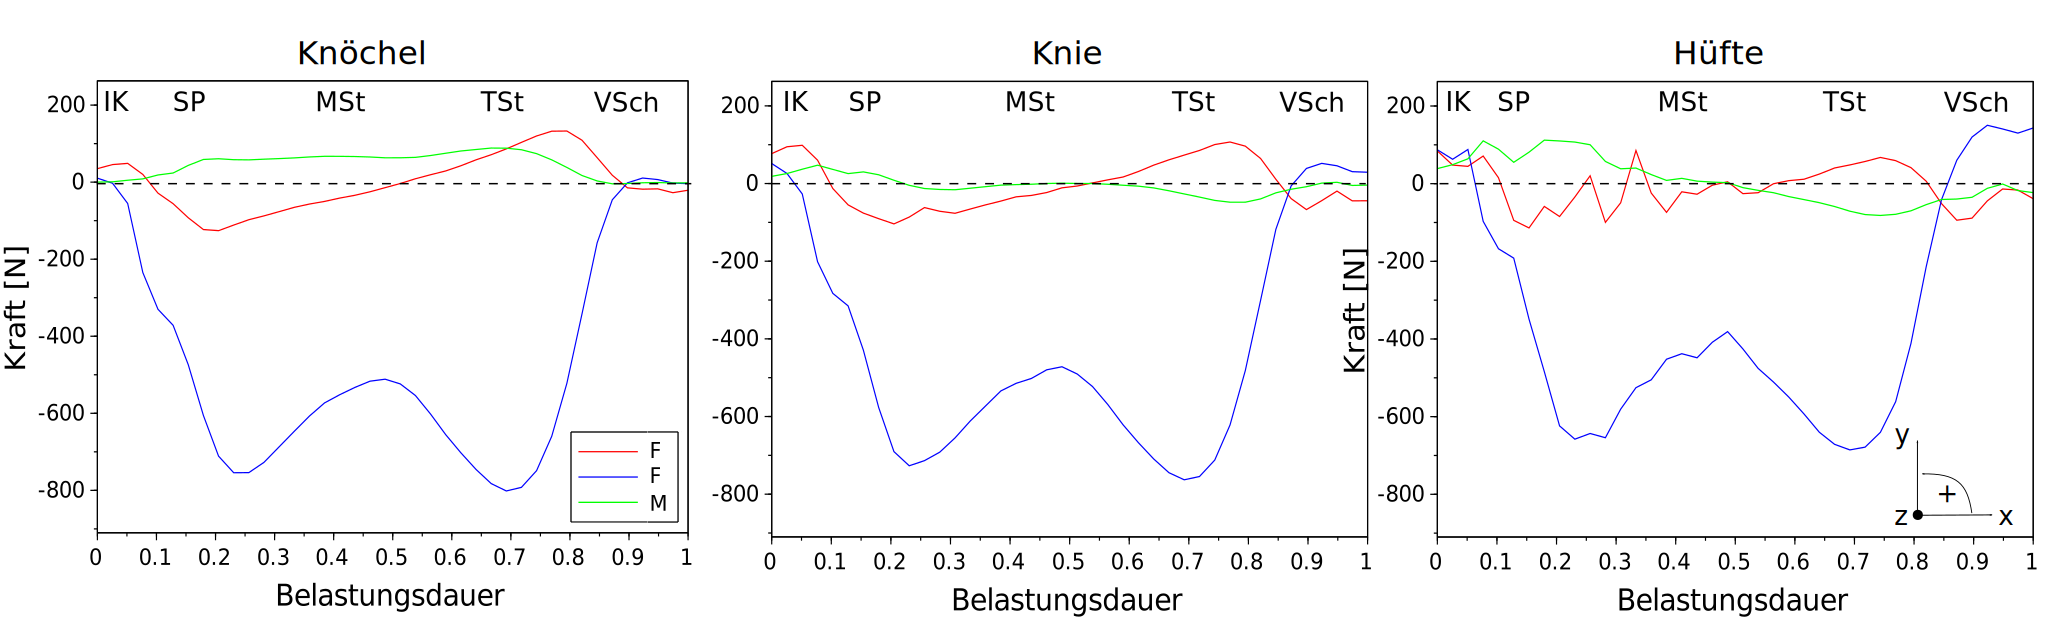
\includegraphics[width=\linewidth]{bilder/Ergebnisse/ang_inv_kin}
	\caption{Kräfte und Momente bei 5~km~h$^{-1}$ in Knöchel-, Knie- und Hüftgelenk}
	\label{fig:ang_inv_kin}
\end{figure}

Wie im vorigen Kapitel sei hier das Knie im Detail mit Fokus auf das Moment dargestellt.
Während das Moment im Knie bei 2~km~h$^{-1}$ nahezu Null ist, ausgenommen zweier kleiner Maxima bei Beginn und Ende des Plateaus der Y-Kraft, zeigt das Moment bei 5~km~h$^{-1}$ deutliche Ausschläge. Während der initialen Kontaktphase und Stoßdämpfungsphase ist das Moment positiv, während es über die mittlere Standphase nahezu Null ist und in der terminalen Standphase einen deutlich negativen Ausschlag hat. Bei 7~km~h$^{-1}$ steigt der positive Ausschlag in der Stoßdämpfungsphase steigt stark an. Das Moment bleibt hier bis kurz vor der terminalen Standphase positiv und hat nur ein sehr geringes negatives Moment in der terminalen Standphase.\\
\begin{figure}[h!]
	\centering
	\includegraphics[width=\linewidth]{bilder/Ergebnisse/comp_knee_mom}
	\caption{Kräfte und Momente im Knie-Gelenk bei 2, 5 und 7~km~h$^{-1}$. Standphasen: Initialer Kontakt IK, Stoßdämpfungsphase SP, mittlere und terminale Standphase MSt bzw. TSt sowie Vorschwungphase VSch}
	\label{fig:comp_knee_mom}
\end{figure}

\subsection{Vergleich Laufband und Laufstrecke}
Die auf der Laufstrecke erreichten Geschwindigkeiten entsprechen 2,1~km~h$^{-1}$ (langsam), 4,9~km~h$^{-1}$ (angenehm) und 6,7~km~h$^{-1}$ (schnell) und werden auf ganzzahlige Geschwindigkeiten gerundet, um die Handtrajektorien, den Winkel der Körperachse und den Kniewinkel auf Laufband und -strecke zu vergleichen.\\
Bei 2~km~h$^{-1}$ ist kein klares Vor- und Zurückschwingen erkennbar und die Hand wird deutlich vor der Körperachse (x~=~0) geführt. Eine deutlichere Schwungbewegung wird bei 5~km~h$^{-1}$ sichtbar. Die X-Amplitude ist auf dem Laufband größer als auf der Laufstrecke. Während die Laufband-Trajektorie vorne abgeflacht ist, beschreibt die Laufstrecken-Trajektorie eine acht. Bei 7~km~h$^{-1}$ steigt die X-Amplitude für beide Versuche weiter an. Beide Trajektorien sind nun flach und weisen in entgegengesetzte Richtungen weisende Krümmungen auf. Der Armschwung findet für Laufband und -strecke vor und hinter der Körperachse statt.\\
Bei allen drei Geschwindigkeiten ist die Körperachse auf dem Laufband mehr nach vorne geneigt als auf der Laufstrecke, bis auf ein Minimum bei 2~km~h$^{-1}$. Während bei 2~km~h$^{-1}$ kein deutliches Schwanken des Winkels der Körperachse um einen Mittelwert zu erkennen ist, kann diese bei 5 und 7~km~h$^{-1}$ deutlich beobachtet werden. Mit dem Wechsel von 5 zu 7~km~h$^{-1}$ verlagert sich der Mittelwert auf dem Laufband von 0$^{\circ}$ zu 2$^{\circ}$, während der Mittelwert für die Laufstrecke von -2$^{\circ}$ auf 0$^{\circ}$ erhöht. Der Körper ist daher auf der Laufstrecke generell weiter nach hinten geneigt als auf dem Laufband.\\
Zum weiteren Vergleich sei hier exemplarisch der Verlauf einer der Gelenkwinkel gezeigt. Der Kniewinkelverlauf ist für den Laufbandversuch über den Doppelschritt dargestellt, während für die Laufstrecke der Fokus aufgrund der inversen Kinetik auf die Standphase gelegt wird.\\
Für alle drei Geschwindigkeiten ist der Verlauf des Winkels auf Laufband und Laufstrecke ähnlich. Für die Sub-Phasen der Standphase wird die Veränderung des Kniewinkels mit der Geschwindigkeit betrachtet. Je schneller der Proband geht, desto stärker ist das Knie gestreckt. Dies ist unabhängig vom Versuch erkennbar durch die kleineren Winkel beim initialen Kontakt (s.~Abb.~\ref{fig:comp_knee_angle}). In der Stoßdämpfungsphase wird das Knie mit steigender Geschwindigkeit deutlich stärker flektiert. Die Flexion steigt von 10$^{\circ}$ beträgt bei 2~km~h$^{-1}$ über 20$^{\circ}$ bei 5~km~h$^{-1}$ auf 26$^{\circ}$ bei 7~km~h$^{-1}$. Bei allen Geschwindigkeiten ist in der mittleren Standphase eine Extension von 16$^{\circ}$ auf dem Laufband und 14$^{\circ}$ auf der Laufstrecke zu beobachten. Der maximale Flexionswinkel wird in der Initialen Schwungphase erreicht und steigt von 63$^{\circ}$ bei 2~km~h$^{-1}$ auf ca. 71$^{\circ}$ bei 5 und 7~km~h$^{-1}$.\\ 

\begin{figure}[h!]
	\centering
	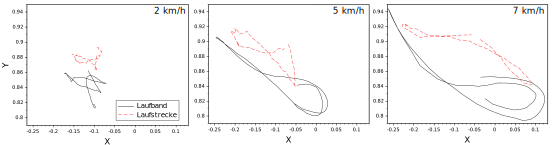
\includegraphics[width=\linewidth]{bilder/Ergebnisse/compare_hand}
	\caption[Handtrajektorien auf dem Laufband und -strecke]{Verlauf der Handtrajektorien auf Laufband und -strecke bei 2, 5 und 7~km~h$^{-1}$. Y-Achse: Höhe über Boden. X-Achse: Auslenkung der Hand. Die Körperachse liegt bei x~=~0.}
	\label{fig:res_compare_hand}
\end{figure}
\begin{figure}[h!]
	\centering
	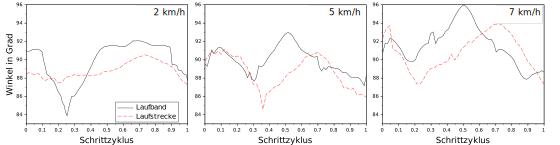
\includegraphics[width=\linewidth]{bilder/Ergebnisse/compare_trunk}
	\caption[Winkelverlauf der Körperachse auf Laufband und -strecke]{Winkelverlauf der Körperachse gegenüber der Horizontalen für Laufband und -strecke bei 2, 5 und 7~km~h$^{-1}$. Aufrechte Körperachse entspricht 0$^{\circ}$, negative Winkel entsprechen zurückgelehnter und positive Winkel vorgebeugter Körperachse}
	\label{fig:res_compare_trunk}
\end{figure}%
\begin{figure}[h!]
	\centering
	\includegraphics[width=\linewidth]{bilder/Ergebnisse/compare_knee_angle_3_speeds}
	\caption{Verlauf des Kniewinkels über Doppelschritt auf dem Laufband und über Standphase auf der Laufstrecke für 2, 5 und 7~km~h$^{-1}$. Gekennzeichnet sind initaler Kontakt (IK) und Lösen der Zehen (LZ)}
	\label{fig:comp_knee_angle}
\end{figure}
